\section{Qualitative figures of the fine-only baseline}
\label{sec:supp_gallery}
These figures show the earlier fine-only pipeline of Sec.~\ref{sec:supp_baseline} (uniform seed, two passes through 64-pixel SA, DenseCRF at 0.45). Figure~\ref{fig:supp_gallery} shows, by a fixed rule, the four classes with the lowest class IoU of that pipeline on each dataset, each shown by its median-IoU image. No image was inspected before the choice. The COCO-Cap columns show three different failures. For the chair, propagation leaks into the wooden wall behind it. For the dining table, which fills the frame, the mask covers the plate and bread on it but not its surface. For the bottle, the mask covers both bottles, but only one is annotated, so part of the error is in the label rather than the mask.

\begin{figure*}[t]
\centering
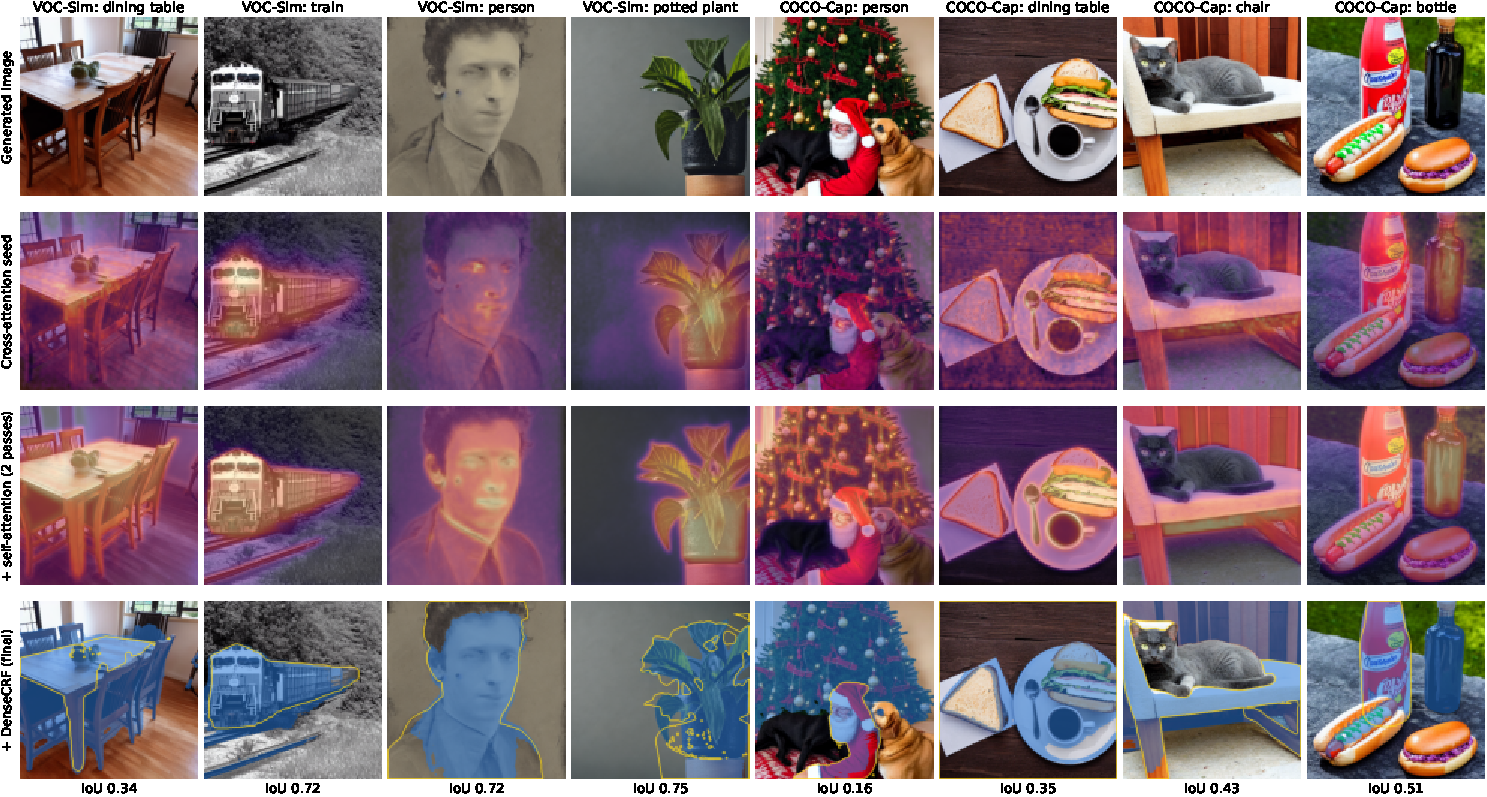
\includegraphics[width=\textwidth]{figures/supp_gallery.pdf}
\caption{\textbf{The weakest classes, one median image each.} Rows: generated image; CA seed; two SA passes; final mask after DenseCRF at 0.45 (blue) with the ground-truth outline (yellow) and the image IoU. Columns: the four lowest class IoUs on VOC-Sim, then on COCO-Cap, from the lowest.}
\label{fig:supp_gallery}
\end{figure*}

\paragraph{CA resolution.} Figure~\ref{fig:supp_ca_example} illustrates the CA resolution decision (Table~2 of the main paper) on one image.

\begin{figure*}[t]
\centering
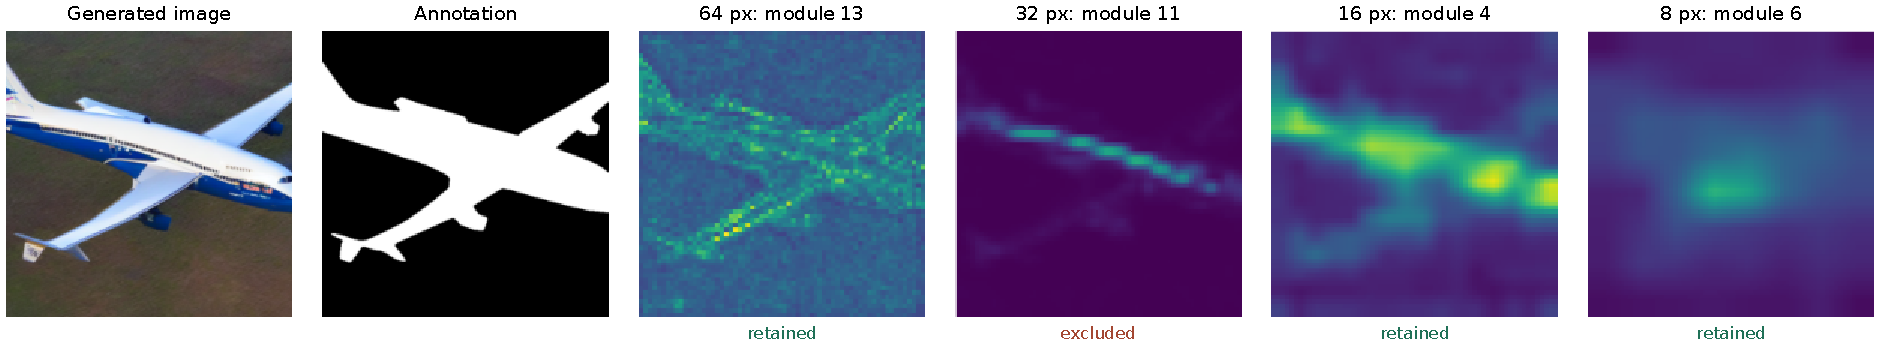
\includegraphics[width=\textwidth]{figures/ca_airplane.pdf}
\caption{\textbf{Why CA resolution is a real design choice.} One VOC-Sim airplane generated image and annotation (left), followed by representative head-averaged CA modules from the same image and all calls. All heatmaps use one color scale. The selected seed retains 8, 16 and 64-pixel modules and omits the 32-pixel group. This visual example motivates the controlled resolution test; the fold-level evidence is in Table~2 of the main paper.}
\label{fig:supp_ca_example}
\end{figure*}

\paragraph{Propagation depth.} Figure~\ref{fig:supp_propagation_depth} applies both selection rules of Fig.~\ref{fig:supp_depth} to both datasets.

\begin{figure*}[t]
\centering
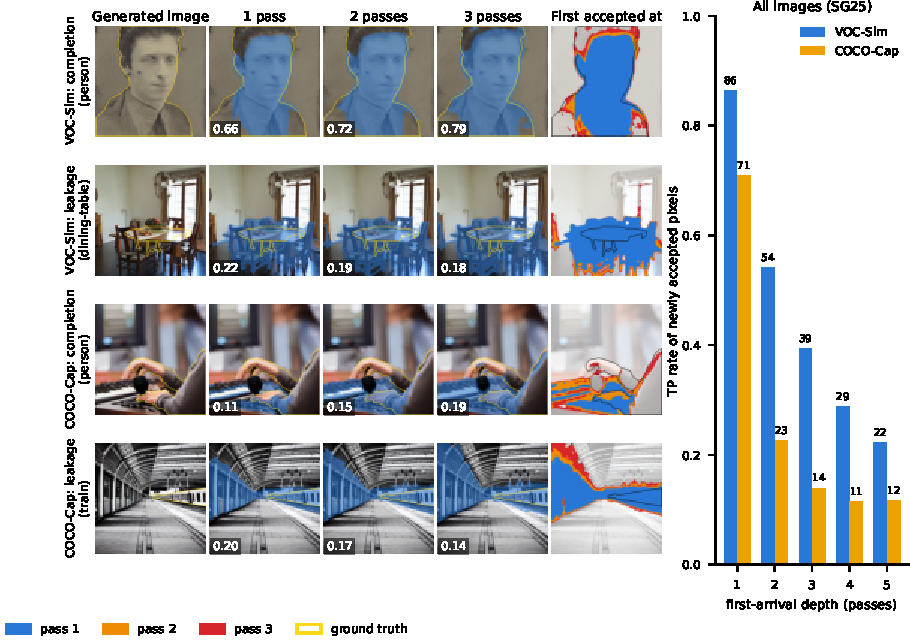
\includegraphics[width=\textwidth]{figures/supp_propagation_depth.pdf}
\caption{\textbf{One, two and three SA passes, both rules on both datasets.} Rows: on each dataset, the image at the 90th percentile of the two-pass gain (completion) and at the 10th percentile of the three-pass gain (leakage), from the all-call raw maps of SG22 at threshold 0.45. Columns and right panel as in Fig.~\ref{fig:supp_depth}.}
\label{fig:supp_propagation_depth}
\end{figure*}
